\documentclass[aspectratio=169]{../latex_main/tntbeamer}  % you can pass all options of the beamer class, e.g., 'handout' or 'aspectratio=43'
\usepackage{dsfont}
\usepackage{bm}
\usepackage[english]{babel}
\usepackage[T1]{fontenc}
%\usepackage[utf8]{inputenc}
\usepackage{graphicx}
\graphicspath{ {./figures/} }
\usepackage{algorithm}
\usepackage[ruled,vlined,algo2e,linesnumbered]{algorithm2e}
\usepackage{hyperref}
\usepackage{booktabs}
\usepackage{mathtools}

\usepackage{amsmath,amssymb}

\DeclareMathOperator*{\argmax}{arg\,max}
\DeclareMathOperator*{\argmin}{arg\,min}

\usepackage{pgfplots}
\pgfplotsset{compat=1.16}
\usepackage{tikz}
\usetikzlibrary{trees} 
\usetikzlibrary{shapes.geometric}
\usetikzlibrary{positioning,shapes,shadows,arrows,calc,mindmap}
\usetikzlibrary{positioning,fadings,through}
\usetikzlibrary{decorations.pathreplacing}
\usetikzlibrary{intersections}
\pgfdeclarelayer{background}
\pgfdeclarelayer{foreground}
\pgfsetlayers{background,main,foreground}
\tikzstyle{activity}=[rectangle, draw=black, rounded corners, text centered, text width=8em]
\tikzstyle{data}=[rectangle, draw=black, text centered, text width=8em]
\tikzstyle{myarrow}=[->, thick, draw=black]

% Define the layers to draw the diagram
\pgfdeclarelayer{background}
\pgfdeclarelayer{foreground}
\pgfsetlayers{background,main,foreground}

% Requires XeLaTeX or LuaLaTeX
\usepackage{unicode-math}

\usepackage{fontspec}
%\setsansfont{Arial}
\setsansfont{RotisSansSerifStd}[ 
Path=../latex_main/fonts/,
Extension = .otf,
UprightFont = *-Regular,  % or *-Light
BoldFont = *-ExtraBold,  % or *-Bold
ItalicFont = *-Italic
]
\setmonofont{Cascadia Mono}[
Scale=0.8
]

% scale factor adapted; mathrm font added (Benjamin Spitschan @TNT, 2021-06-01)
%\setmathfont[Scale=1.05]{Libertinus Math}
%\setmathrm[Scale=1.05]{Libertinus Math}

% other available math fonts are (not exhaustive)
% Latin Modern Math
% XITS Math
% Libertinus Math
% Asana Math
% Fira Math
% TeX Gyre Pagella Math
% TeX Gyre Bonum Math
% TeX Gyre Schola Math
% TeX Gyre Termes Math

% Literature References
\newcommand{\lit}[2]{\href{#2}{\footnotesize\color{black!60}[#1]}}

%%% Beamer Customization
%----------------------------------------------------------------------
% (Don't) Show sections in frame header. Options: 'sections', 'sections light', empty
\setbeamertemplate{headline}{empty}

% Add header logo for normal frames
\setheaderimage{
	% 
\includegraphics[height=\logoheight]{figures/TNT_darkv4.pdf}
	
\includegraphics[height=\logoheight]{../latex_main/figures/luh_logo_rgb_0_80_155.pdf}
	% 
\includegraphics[height=\logoheight]{figures/logo_tntluh.pdf}
}

% Header logo for title page
\settitleheaderimage{
	% 
\includegraphics[height=\logoheight]{figures/TNT_darkv4.pdf}
	
\includegraphics[height=\logoheight]{../latex_main/figures/luh_logo_rgb_0_80_155.pdf}
	% 
\includegraphics[height=\logoheight]{figures/logo_tntluh.pdf}
}

% Title page: tntdefault 
\setbeamertemplate{title page}[tntdefault]  % or luhstyle
% Add optional title image here
%\addtitlepageimagedefault{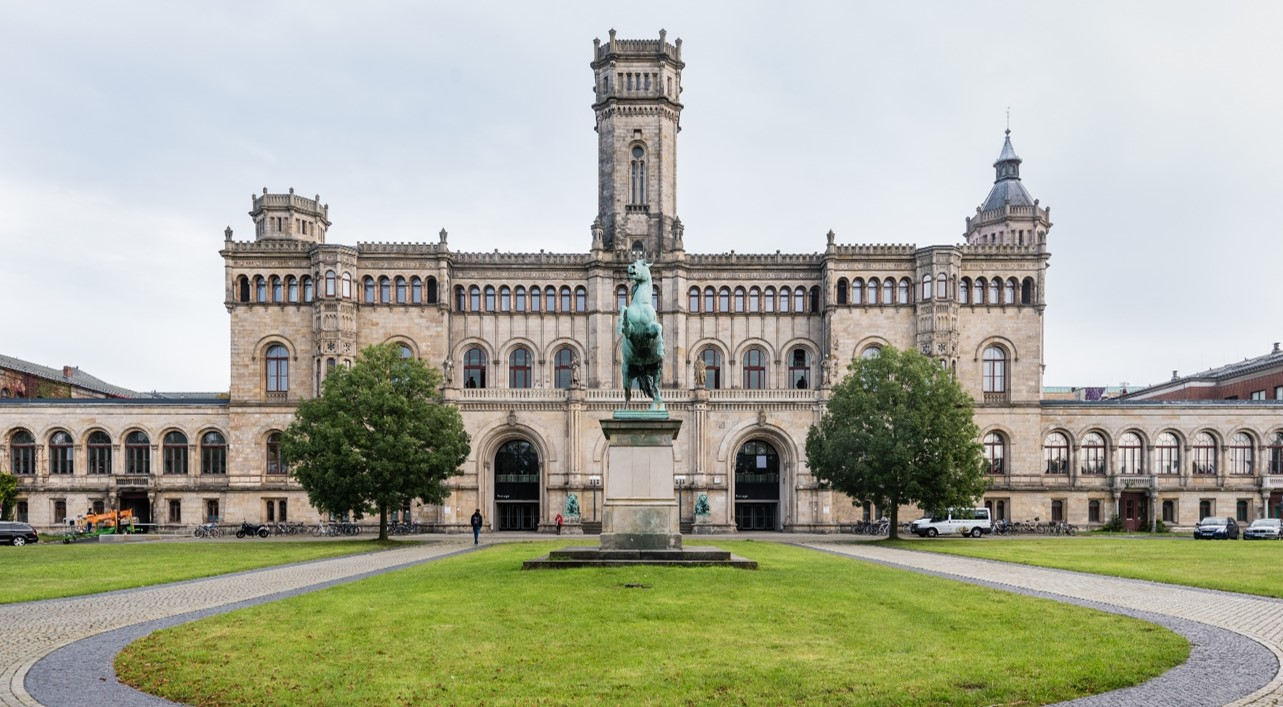
\includegraphics[width=0.65\textwidth]{figures/luh_default_presentation_title_image.jpg}}

% Title page: luhstyle
% \setbeamertemplate{title page}[luhstyle]
% % Add optional title image here
% \addtitlepageimage{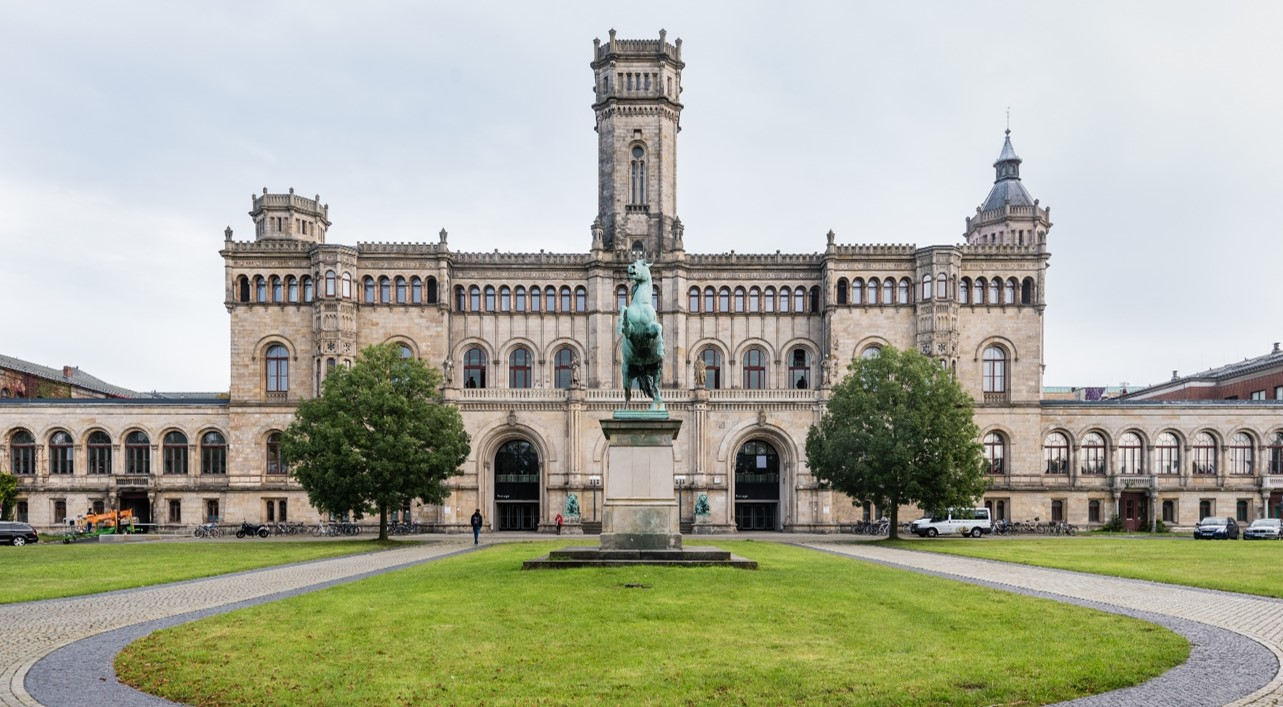
\includegraphics[width=0.75\textwidth]{figures/luh_default_presentation_title_image.jpg}}

\author[Lindauer \& Anand]{Marius Lindauer and Avishek Anand\\[1em]
	
\includegraphics[height=\logoheight]{../latex_main/figures/luh_logo_rgb_0_80_155.pdf}\qquad

\includegraphics[height=\logoheight]{../latex_main/figures/TNT_darkv4}\qquad

\includegraphics[height=\logoheight]{../latex_main/figures/L3S.jpg}	}
\date{Winter Term 2021
}


%%% Custom Packages
%----------------------------------------------------------------------
% Create dummy content
\usepackage{blindtext}

% Adds a frame with the current page layout. Just call \layout inside of a frame.
\usepackage{layout}


\title[Introduction]{iML: Shapley Values}
\subtitle{Introduction}

%\institute{}


\begin{document}
	
	\maketitle
	
	\begin{frame}[c]{Example}
	
	\begin{itemize}
	    \item Exemplary model for predicting apartment price
	    \item Inputs
	    \begin{itemize}
	        \item Size (m$^2$)
	        \item location (e.g., floor)
	        \item close by (e.g., train station)
	        \item pets allowed?
	    \end{itemize}
	    \item Average apartment price is 310k
	    \pause
	    \bigskip
	    \item Query: 50m$^2$, 2nd floor, park close by, pets not allowed
	    \item Prediction: 300k
	    \item[$\leadsto$] Why?
	\end{itemize}
	
	\end{frame}

\begin{frame}[c]{Example (cont'd)}
	
	\begin{itemize}
	    \item Query: 50m$^2$, 2nd floor, park close by, pets not allowed
	    \item Prediction: 300k
	    \item[$\leadsto$] Why?
	    \bigskip
        \item Possible approaches: linear models or LIME
        \item \alert{New question:} Under all possible subsets of features, how much would feature $S$ contribute to the prediction?
	\end{itemize}
	
\end{frame}

\begin{frame}[c]{Shapley Values}
	
	\begin{itemize}
	    \item Origin in game theory \lit{Shapley 1953}{}
	    \begin{itemize}
	        \item How much does a player contributes to the total payout (i.e., gain) under different coalitions with other players?
	    \end{itemize}
	    \pause
	    \item Relation to iML:
	    \begin{itemize}
	        \item Game: Prediction task
	        \item Players: Features values of the instance 
	        \item Gain: Difference between actual prediction and average prediction $\leadsto$ -10k in our example
	    \end{itemize}
    	\pause
    	\smallskip
    	\item The answer could be: park close by $\leadsto$ 30k, 50m$^2$ $\leadsto$ 10k, 2nd floor $\leadsto$ 0k, pets banned $\leadsto$ -50k
    	\pause
    	\smallskip
    	\item[$\leadsto$] Shapley value: Average marginal contribution of a feature value across all possible coalitions.
	\end{itemize}
\end{frame}

\begin{frame}[c]{Shapley Values: In a Nutshell}
	
	\begin{itemize}
	    \item For all possible subsets of features (i.e., coalition):
	    \begin{enumerate}
	        \item add feature value under consideration to the coalition once and once a random value
	        \item randomly change features not being in the coalition for both samples
	        \item predict difference between both samples
	        \item[$\leadsto$] marginal contribution of feature to coalition
	    \end{enumerate}
	    
	 \end{itemize}
\end{frame}

\begin{frame}[c]{Shapley Values: Continued example}
	
	\begin{itemize}
	    \item Possible coalition for example if we consider \alert{pet}:
	    \begin{itemize}
	        \item $\emptyset$ (no features)
	        \item size
	        \item location
	        \item close-by
	        \item size + location
	        \item size + close-by
	        \item location + close-by
	        \item size + location + close-by
	    \end{itemize}
	    
	 \end{itemize}
\end{frame}

\begin{frame}[c]{Shapley Values: Continued example}
	
	\begin{itemize}
	    \item Exemplary coalition: size
	    \item Considered feature value: pets banned
	    \item considered, randomly sampled feature vectors:
	    \begin{enumerate}
	        \item size:50, pets:banned, location: 3rd, close-by:train-station\\
	        size:50, pets:allowed, location: 3rd, close-by:train-station\\
	        \item size:50, pets:banned, location: 1st close-by:park\\
	        size:50, pets:allowed, location: 1st, close-by:park\\
	        \item \ldots
	    \end{enumerate}
	 \end{itemize}
\end{frame}

\end{document}
